\pgfdeclarelayer{pre main}
\pgfdeclarelayer{background}
\pgfdeclarelayer{foreground}
\pgfsetlayers{background,pre main,main,foreground} 
% Декорация линий
\tikzset{
	% декорация линий
	curve line/.style={
		decoration={
			snake,
			amplitude=1.5mm,%0.75mm,
			segment length=7.5mm,
			post length=0mm,
			pre length=0mm,
		},
	},
	pointnode/.style={
		join=by -,
		circle,
		fill=red,
		minimum size=3pt,
		inner sep=0pt,
	},
	circlenode/.style={
		draw,thick,fill=blue!10,line width=0.25mm,
		shape=circle,
		inner sep=4pt,
	},
	rectnode/.style={
		draw,line width=0.25mm,
		shape=rectangle,
%		rounded corners=2pt, 
		inner sep=8pt,
	},
	rrectnode/.style={
		draw,line width=0.25mm,
		shape=rounded rectangle,
%		rounded corners=2pt, 
		inner sep=8pt,
	},
	datanode/.style={
		draw,line width=0.25mm,
		shape=	trapezium,
		trapezium left angle=70,
		trapezium right angle=110, 
		text centered,
		inner sep=8pt,
	},
	ifthenelsenode/.style={
		draw,line width=0.25mm,
		shape=diamond,
		aspect=2,
%		trapezium left angle=70,
%		trapezium right angle=110, 
		text centered,
		inner sep=4pt,
	},
	startloopnode/.style={
		draw,text width=4cm,align=center,line width=0.25mm,
		shape=chamfered rectangle,
		chamfered rectangle corners={north west,north east},
		minimum height=3em,minimum width=5cm,
	},
	endloopnode/.style={
		draw,text width=4cm,align=center,line width=0.25mm,
		shape=chamfered rectangle,
		chamfered rectangle corners={south west,south east},
		minimum height=3em,minimum width=5cm,
	},
	signalnode/.style={
		draw,line width=0.25mm,
		shape=chamfered rectangle,
		chamfered rectangle angle=45,
		chamfered rectangle xsep=1cm,
		inner sep=8pt,
	},
}

\newpage

\section{Методы локальной оптимизации}

Оптимизация -- это задача нахождения экстремума 
(минимума или максимума) целевой функции в некоторой области 
конечномерного векторного пространства, ограниченной 
набором линейных и/или нелинейных равенств и/или неравенств.

Во многих практически важных случаях для целевой функции 
многих переменных $f(\vect{x})$ 
задача оптимизации может быть сформулирована в виде:
\begin{gather*}
f(\vect{x})\to\min,
\end{gather*}
где $\vect{x}=(x_1,x_2,\ldots,x_n)$ --
вектор неизвестных (управляющих параметров);\linebreak
$\min$ -- минимальное значение функции в ограниченной 
или неограниченной области изменения неизвестных.

Для нахождения абсолютного минимума целевой функции $f(\vect{x})$
существует только один способ: 
найти все локальные минимумы этой функции, 
сравнить их и выбрать из них тот,
в котором функция принимает наименьшее значение.

% Минимум функции одного переменного 
% http://www.machinelearning.ru/wiki/index.php?title=%D0%9C%D0%B5%D1%82%D0%BE%D0%B4_%D0%B7%D0%BE%D0%BB%D0%BE%D1%82%D0%BE%D0%B3%D0%BE_%D1%81%D0%B5%D1%87%D0%B5%D0%BD%D0%B8%D1%8F._%D0%A1%D0%B8%D0%BC%D0%BC%D0%B5%D1%82%D1%80%D0%B8%D1%87%D0%BD%D1%8B%D0%B5_%D0%BC%D0%B5%D1%82%D0%BE%D0%B4%D1%8B
\emptyline
\subsection{Минимум функции одного переменного}
Для функции одной переменной $f(x)$, задача нахождения минимума
эквивалента задачи нахождения корней уравнения:
\begin{equation}\label{eq:GD:f(x)=min}
\diff{f(x)}{x}=0
\end{equation}

Эта одномерная задача нередко возникает в практических 
приложениях. Кроме того, большинство методов решения 
многомерных задач сводится к поиску одномерного минимума. 

Предположим, что $f(x)$ задана и кусочно-непрерывна на отрезке 
$x\in[a,b]$, и имеет на этом отрезке (включая его концы) 
только один локальный минимум. 
Построим итерационный процесс, сходящийся к этому минимуму. 

Вычислим значение функции на концах отрезка $x=a$ и $x=b$, 
а также в двух внутренних точках $x_1<x_2$.
Так так функция $f(x)$ имеет минимум на отрезке $x\in[a,b]$, 
то справедливо утверждение:
\begin{equation*}
f(a)\geqslant f(x_1),\quad f(x_2)\leqslant f(b)
\end{equation*}

Сравним все четыре значения функции между собой 
$f(a)$, $f(x_1)$, $f(x_2)$ и $f(b)$ и выберем среди них наименьшее.

%
%	График функций
%
\begin{figure}[H]\centering
\begin{tikzpicture}
\begin{axis}
[
xlabel={\empty},	% подпись оси x
ylabel={$f(x)$},	% подпись оси y
enlargelimits=true,
xmin=0, xmax=3, xtick={0,0.75,2.25,3}, xticklabels={$a$,$x_1$,$x_2$,$b$},
ymin=0, ymax=2, ytick={1,{0.25^2},{1+ln(2.25-0.75)},{1+ln(3-0.75)}}, yticklabels={},
%ytick={\empty}
]
\path[name path=O] (axis cs:0,0) -- (axis cs:2.25,0);
% функция f(x)
\addplot[name path=A1,thick,color=darkred,domain=0:1.5, samples=50] {(x-1)^2};
\addplot[name path=A2,thick,color=darkred,domain=1.5:3, samples=50] {1+ln(x-0.75)};
% область
\addplot [orange!15] fill between [of=A1 and O, soft clip={domain=0:1.5}];
\addplot [orange!15] fill between [of=A2 and O, soft clip={domain=1.5:2.25}];
% маркеры
\addplot[only marks,ball darkred] coordinates{(0,1)}
node[above]{$f(a)$};
\addplot[only marks,ball darkred] coordinates{(3,{1+ln(3-0.75)})}
node[above]{$f(b)$};
\addplot[only marks,ball darkblue] coordinates{(0.75,{0.25^2})}
node[above right]{$f(x_1)$};
\addplot[only marks,ball darkblue] coordinates{(2.25,{1+ln(2.25-0.75)})}
node[below right]{$f(x_2)$};
\end{axis}
\end{tikzpicture}
\caption{График кусочно-непрерывной функции $y=f(x)$,\linebreak
имеющей минимум на отрезке $x\in[a,b]$}
\label{fig:GD:f(x)=min}
\end{figure}

Из рисунка \ref{fig:GD:f(x)=min} видно, что наименьшее значение
функция достигает в точке $x=x_1$:
\begin{equation*}
f(x_1)<f(a)<f(x_2)<f(b)
\end{equation*}

Очевидно, что минимум функции $f(x)$ расположен в одном 
из прилегающих к точке $x=x_1$ отрезков, то есть минимум 
находится либо в пределах отрезка $[a,x_1]$, либо в $[x_1,x_2]$
(рисунок \ref{fig:GD:f(x)=min}, выделенная область).

Поэтому на первом шаге итерационного процесса 
отбрасывается отрезок $[x_2,b]$, и для поиска 
минимума функции $f(x)$ рассматривается отрезок $[a,x_2]$,
при этом область поиска минимума функции сужается:
\begin{equation*}
\abs{a-x_2}<\abs{a-b},\quad\text{так как}\quad x_2<b.
\end{equation*} 

Полагая $b=x_2$, на новом отрезке $[a, b]$ вновь необходимо 
выбрать две внутренние точки, вычислить в них и 
на концах отрезка значения функции $f(x)$, 
и сделать следующий шаг итерационного процесса.

Критерием остановки итерационного процесса является условие выполнения
неравенства, которое гарантирует малость размера области поиска
минимума по сравнению с заранее заданной погрешность метода:
\begin{equation*}
(b-a)\leqslant\epsilon,
\end{equation*}
где $\epsilon$ -- погрешность метода.

\emph{Симметричный метод} поиска минимума функции 
одной переменной $f(x)$ основан на выборе внутренних точек 
$x_1$ и $x_2$ отрезка $[a,b]$, 
которые равноудалены от концов этого отрезка.
Например, если точки $x_1$ и $x_2$ делят отрезок $[a,b]$
на три равные части (рисунок \ref{fig:GD:ab}), 
то координаты этих точек могут быть 
определены из соотношений:
\begin{equation*}
x_1=a+\dfrac{b-a}{3}=\dfrac{2a+b}{3},
\quad
x_2=b-\dfrac{b-a}{3}=\dfrac{a+2b}{3}.
\end{equation*}

\begin{figure}[H]\centering
\begin{tikzpicture}
[>={Straight Barb[angle=45:2mm 1]},shorten >=1pt,font=\small]% стрелка
% начало отсчета
\coordinate (O) at (0mm,0mm);
% ось OX
\draw[->,line width=0.25mm] ([xshift=-20mm]O) -- (80mm,0mm)
node[pos=1,yshift=-1em]{$x$};
% сетка
\coordinate (p) at (O);
\foreach \x [count=\n from 0] in {0,20,20,20}{
\path (p) -- ++(\x mm,0mm) coordinate(p);
\draw[fill=black] (p) circle[radius=0.8mm] coordinate(p\n);
}
% подписи
\draw (p0) node[above]{$a$};
\draw (p1) node[above]{$x_1$};
\draw (p2) node[above]{$x_2$};
\draw (p3) node[above]{$b$};
% штриховка
\begin{scope}[on background layer]
\pattern[pattern=north east lines,pattern color=gray,opacity=0.75]
(p0) -- ([yshift=-2mm]p0) -- ([yshift=-2mm]p3) -- (p3) -- cycle;
\end{scope}
\end{tikzpicture}
\caption{Схематическое изображение точек деления отрезка $[a,b]$}
\label{fig:GD:ab}
\end{figure}

Оценка длины отрезка после первого итерационного шага составит:
\begin{equation*}
\ell_1=(b-a) - \dfrac{b-a}{3}=\dfrac{2}{3}\cdot(b-a),
\end{equation*}
после второго шага:
\begin{equation*}
\ell_2=\ell_1-\dfrac{\ell_1}{3}=\dfrac{2}{3}\cdot\ell_1=
\left(\dfrac{2}{3}\right)^2\cdot(b-a),
\end{equation*}
а после $k$-ого итерационного шага:
\begin{equation*}
\ell_k=\left(\dfrac{2}{3}\right)^k\cdot(b-a).
\end{equation*}

Таким образом, чтобы погрешность вычисления 
$\ell_k$ была менее $\epsilon$, для числа итераций $k$ 
справедлива оценка:
\begin{equation*}
\left(\dfrac{2}{3}\right)^k\cdot(b-a)\leqslant\epsilon
\quad\to\quad
k=\left\lceil\dfrac{\ln(b-a)-\ln(\epsilon)}{\ln(3)-\ln(2)}\right\rceil
\end{equation*}

Симметричный метод поиска минимума функции является 
аналогом метода дихотомии для нахождения корня уравнения $f(x)=0$. 
Метод применим к недифференцируемым функциям и всегда 
сходится. 
Следует отметить, что если на отрезке $[a,b]$
функция $f(x)$ имеет несколько локальных минимумов, 
то итерационный процесс сойдется к одному из этих минимумов, 
но не обязательно к наименьшему. 

% *** Алгоритм поиска минимума функции одной переменной
% https://tex.stackexchange.com/questions/370704/drawing-a-scheme
\begin{figure}[H]\centering
\begin{tikzpicture}[
font=\small,
start chain=going below,node distance=10mm,every join/.style=->,%
>={Straight Barb[angle=45:1.5mm 1]},shorten >=0.5pt,%
]
% соединитель
\node[rrectnode,on chain,join]{старт};
% данные
\node[datanode,on chain,join]
{$a, b, \epsilon$};
% x1, x2
\node[rectnode,on chain,join](x1x2)
{$x_1=\dfrac{2a+b}{3},\;x_2=\dfrac{a+2b}{3}$};
% f(x1) < f(x2)
\node[ifthenelsenode,on chain,join,fill=gray!10](compare)
{$f(x_1)>f(x_2)$};
% да
\begin{scope}[start branch=a,node distance=15mm]
\node[rectnode,on chain=going left,join](a)
{$a=x_1$};
\draw(compare.west) node[above left]{да};
\end{scope}
% нет
\begin{scope}[start branch=b,node distance=15mm]
\node[rectnode,on chain=going right,join](b)
{$b=x_2$};
\draw(compare.east) node[above right]{нет};
\end{scope}
% ошибка
\node[rectnode,on chain](error)
{$\Delta=b-a$};
% связи
\draw[->] (a.south) |- (error.west);
\draw[->] (b.south) |- (error.east);
% выход?
\node[ifthenelsenode,on chain,join,fill=red!10](exit)
{$\Delta<\epsilon$};
\draw (exit.east) node[above right,darkred]{нет};
\draw[->,darkred,thick] (exit.east) -- ([xshift=5cm]exit.east) |- (x1x2.east);
% соединитель
\draw (exit.south) node[below left]{да};
\begin{scope}[node distance=12mm]
\node[rrectnode,on chain,join]{стоп};
\end{scope}
\end{tikzpicture}
% *******************************************
\caption{Блок-схема алгоритма нахождения минимума\linebreak 
функции $f(x)$ одного переменного}
\label{fig:GD:scheme f(x)->min}
\end{figure}

%
% Минимум функции многих переменных
%
\emptyline
\subsection{Минимизация функций многих переменных}

Задача безусловной минимизации (оптимизации) 
состоит в нахождении минимума или максимума функции $f(\vect{x})$
в отсутствие каких-либо ограничений на область изменения
переменных задачи $\vect{x}\in(-\infty,+\infty)$.

Большинство практических задач оптимизации 
содержит ограничения, которые обусловлены 
технико-экономическим смыслом решаемой задачи,
однако многие алгоритмы решения задач с ограничениями 
предполагают сведение ее к последовательности задач 
безусловной оптимизации.

% Спуск по координатам
\emptyline
\subsubsection{Спуск по координатам}
Идея метода по координатного спуска заключается в том, что
задача поиска минимума функции $f(x_1,x_2,\ldots,x_n)\to\min$
разделяется на серию задач \alert{одномерной минимизации} 
этой функции вдоль направления одной из координатных осей:
\begin{equation*}
\begin{matrix}
f(\textcolor{darkred}{x_1},x_2=\const,\ldots,x_n=\const)\to\min\\
f(x_1=\const,\textcolor{darkred}{x_2},\ldots,x_n=\const)\to\min\\
\hdotsfor{1}\\
f(x_1=\const,x_2=\const,\ldots,\textcolor{darkred}{x_n})\to\min\\
\end{matrix}
\end{equation*}

\begin{enumerate}
\item
Выбирают нулевое приближение 
$\vect{x}_0=(x_{10},x_{20},\ldots,x_{n0})$.
\item
Фиксируют (считают постоянными)  значения всех 
координат кроме $x_1$. Тогда функция $f(\vect{x})$
будет зависеть только от одной переменной $x_1$:
\begin{equation*}
\phi_1(x_1)=f(x_1,x_{20}=\const,\ldots,x_{n0}=\const)
\end{equation*}
\item
Используя метод одномерной минимизации, находится 
минимум функции одной переменной $\phi_1(x_1)\to\min$, 
который можно обозначить через $m_1$.
\item
Сделан переход из начальной точки $\vect{x}_0$ в точку
``частного`` минимума по направлению, параллельному оси $x_1$:
\begin{equation*}
(x_{10},x_{20},\ldots,x_{n0})\to(m_1,x_{20},\ldots,x_{n0}),
\end{equation*}
и значение функции уменьшается:
\begin{equation*}
f(x_{10},x_{20},\ldots,x_{n0})>f(m_1,x_{20},\ldots,x_{n0})
\end{equation*}
\item
Затем из новой точки $(m_1,x_{20},\ldots,x_{n0})$
осуществляется спуск по направлению, параллельному оси $x_2$,
то есть находится минимум функции: 
\begin{equation*}
\phi_2(x_2)=f(m_1=\const,x_2,\ldots,x_n=\const),
\end{equation*}
который обозначим $m_2$.
\item
Таким образом, сделан переход во вторую точку
``частного`` минимума по направлению, параллельному оси $x_2$:
\begin{equation*}
(m_1,x_{20},\ldots,x_{n0})\to(m_1,m_2,\ldots,x_{n0}),
\end{equation*}
и значение функции уменьшается:
\begin{equation*}
f(m_1,x_{20},\ldots,x_{n0})>f(m_1,m_2,\ldots,x_{n0})
\end{equation*}
\item
Процесс спуска по координатам повторяется для всех переменных
задачи $x_3,x_4,\ldots,x_n$, а приход в точку 
$\vect{x}_m=(m_1,m_2,\ldots,m_n)$ завершает цикл спусков.
\item
Конечную точку цикла спусков можно принять за нулевое 
приближение\linebreak $\vect{x}_0=\vect{x}_m$ 
и повторить цикл спусков по координатам $x_1,x_2,\ldots,x_n$
до тех пока, не выполнено условие останова 
итерационного процесса.
\end{enumerate}

\emptyline
Практически можно задать некоторое число $\varepsilon > 0$, 
связанное с выбранной точностью вычислений, и 
проводить итерации до тех пор, пока на $k$-ой итерации
не будут выполнены одно или несколько неравенств вида:
\begin{equation}
\norma{\vect{x}_k - \vect{x}_{k-1}} < \varepsilon_1,
\quad
\norma{f(\vect{x}_k)-f(\vect{x}_{k-1})} < \varepsilon_2
\end{equation}

%
% 3D-график
%
\begin{figure}[H]\centering
\begin{subfigure}[b]{.5\linewidth}\centering
\begin{tikzpicture}[
declare function={
	myfunc(\x,\y) = {1 - exp(-(x-1)^2-(y-2)^2)};
}
]
\begin{axis}[
ylabel={$y$},zlabel={$f$},
view={30}{30},%colorbar,
xtick=\empty,ytick=\empty,ztick=\empty,
axis lines=center,axis on top,
colormap/blackwhite,
z buffer=sort,
]
% целевая функция
\addplot3[surf,opacity=0.75,thin,
domain=-1:3,y domain=0:4,samples=20,
]{1-exp(-(x-1)^2-(y-2)^2)};
% начальная точка
\addplot3[only marks,ball darkblue]
({-0.5},{3},{1-exp(-(-0.5-1)^2-(3-2)^2)})
node[left]{$(x_0,y_0)$};
\end{axis}
\end{tikzpicture}
\end{subfigure}% ВАЖНО!
%
\begin{subfigure}[b]{.5\linewidth}\centering
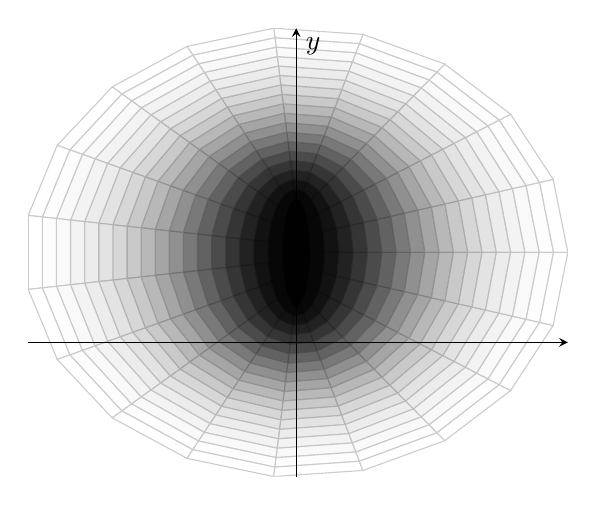
\begin{tikzpicture}
\begin{axis}[
ylabel={$y$},zlabel={$f(x,y)$},
view={0}{90},%colorbar,
xtick=\empty,ytick=\empty,ztick=\empty,
axis lines=center,axis on top,
colormap/blackwhite,
z buffer=sort,
]
\addplot3[surf,opacity=1,thin,
domain=0:2,y domain=0:360,samples=20,
]({x*cos(y)},{1+(0.5+x)*sin(y)},{1-exp(-x^2)});
\end{axis}
\end{tikzpicture}
\end{subfigure}
\caption{График функции $f(x,y)=1-x\cdot e^{-(x-1)^2-y^2}$}
\end{figure}
    

% Метод градиентного спуска
\emptyline
\subsubsection{Метод градиентного спуска}
Градиентный спуск -- метод нахождения локального экстремума 
(минимума или максимума) функции многих переменных 
$f(x_1,x_2,\ldots,x_n)$
с помощью движения вдоль градиента этой функции. 
Это наиболее простой в реализации из всех методов локальной оптимизации, но имеет
относительно малую (линейную) скорость сходимости.

Градиент $\nabla$ это вектор, указывающий направление 
наибольшего возрастания некоторой функции
$f$, значение которой меняется от одной точки 
пространства к другой (скалярного поля), 
а по величине (модулю) равный скорости роста этой величины 
в этом направлении.
Компонентами вектора градиента являются частные производные 
$f$ по всем её аргументам:
\begin{equation}\label{eq:GD:nabla}
\nabla{f}=\left(\pdiff{f}{x_1},\pdiff{f}{x_2},\ldots,\pdiff{f}{x_n}\right)
\end{equation}

Для случая трёхмерного пространства градиентом 
скалярной функции\linebreak
$f(x,y,z)$ называется векторная функция:
\begin{gather*}
\mathrm{grad}\,f=\nabla{f},
\end{gather*}
где $\nabla$ -- векторный дифференциальный оператор набла,
компоненты которого являются частными производными 
по координатам:
\begin{gather*}
\nabla=\left(\pdiff{}{x}, \pdiff{}{y}, \pdiff{}{z}\right)
\end{gather*}

Следует отметить, что оператор набла не принадлежит тому же 
пространству, что и обычные векторы, а говоря точнее, 
скалярное и векторное произведение для него 
определено с некоторыми отличиями. 
Оператор $\nabla$ действует на те скалярные поля, 
что стоят от него справа, и не действует на стоящие от него слева.
Поэтому скалярное и векторное произведение с участием 
$\nabla$ \emph{не коммутативны} и не антикоммутативны, 
как это свойственно для таких произведений обычных векторов.

Минимизация целевой функции $f(\vect{x})$ 
сводится к итерационному процессу 
последовательного выбора нового 
вектора неизвестных $\vect{x}_{k+1}$, такого чтобы
значение функции в новой точки было меньше чем в предыдущих:
\begin{equation*}
f(\vect{x}_0)>f(\vect{x}_1)>\ldots>f(\vect{x}_k)>f(\vect{x}_{k+1})>\ldots
\end{equation*}

Предполагая, что новый вектор неизвестных мало отличается 
от предыдущего ($\vect{x}_{k+1}-\vect{x}_k\approx\vect{0}$),
можно воспользоваться линейным приближением
для разложения в ряд Тейлора целевой функции:
\begin{equation}\label{eq:GD:Taylor}
f(\vect{x}_{k+1}) = f(\vect{x}_k)
+\left(\nabla{f}(\vect{x}_k),\vect{x}_{k+1}-\vect{x}_k\right),
\end{equation}
где $k$ -- номер итерационного шага процесса;
$\vect{x}_k$ -- значение неизвестных на $k$-ой итерации.

Если в качестве нового вектора неизвестных выбрать:
\begin{equation}\label{eq:GD:x(k+1)}
\vect{x}_{k+1}=\vect{x}_k - \lambda\cdot\nabla{f(\vect{x}_k)},
\end{equation}
то из \eqref{eq:GD:Taylor} получим:
\begin{equation}
f(\vect{x}_{k+1}) = f(\vect{x}_k)
-\lambda\cdot\norma{\nabla{f}(\vect{x}_k)}^2
\quad\to\quad
f(\vect{x}_{k+1}) \leqslant f(\vect{x}_k)
\end{equation}
где $\lambda>0$ -- малое положительное число (параметр метода), 
имеющий смысл скорости градиентного спуска;
$\norma{\nabla{f}(\vect{x}_k)}\geqslant0$ -- 
норма вектора градиента (неотрицательное число):
\begin{equation*}
\norma{\nabla{f}}=\sqrt{\left(\nabla{f},\nabla{f}\right)}
\end{equation*}

Таким образом, выбор нового вектора неизвестных $\vect{x}_{k+1}$
в соответствии с выражением \eqref{eq:GD:x(k+1)}, гарантирует
монотонное убывание целевой функции $f(\vect{x})$ в каждой итерации.
Поэтому основная идея метода градиентного спуска заключается в том, 
чтобы последовательно идти в направлении наибольшего
уменьшения целевой функции, которое задаётся антиградиентом 
$-\nabla{f}(\vect{x})$.

% Алгоритм метода градиентного спуска
%\textbf{Алгоритм метода градиентного спуска}
%\begin{enumerate}
%\item 
%Задают начальное приближение ${(x_0,y_0)}$, 
%скорость градиентного спуска $\lambda$, 
%а также точность расчёта $\varepsilon$.
%\item
%Рассчитывают градиент целевой функции
%в текущей точке $\nabla_0=\nabla f(x_0,y_0)$.
%\item
%Определяют новый вектор неизвестных 
%в соответствии с соотношением \eqref{eq:GD:x(k+1)}:
%\begin{gather*}
%\left\{\begin{matrix}
%x_1&=&x_0 - \lambda\cdot{\nabla_0}_x\\
%y_1&=&y_0 - \lambda\cdot{\nabla_0}_y\\
%\end{matrix}\right.,
%\end{gather*}
%где ${\nabla_0}_x$ и ${\nabla_0}_y$ --
%компоненты вектора градиента в выбранной системе координат.
%\item
%Рассчитывают величину расстояния между двумя точками:
%\begin{gather*}
%r=\sqrt{(x_0-x_1)^2+(y_0-y_1)^2}
%\end{gather*}
%\item
%Проверяют условие остановки итерационного процесса:
%если $r<\varepsilon$, то итерационный процесс останавливается;
%иначе текущую точку считают начальной 
%$x_0=x_1$ и $y_0=y_1$ и переходят к шагу (2) 
%итерационного процесса.
%\end{enumerate}


% *** Алгоритм поиска минимума функции одной переменной
% https://tex.stackexchange.com/questions/370704/drawing-a-scheme
\begin{figure}[H]\centering
\begin{tikzpicture}[
font=\small,
start chain=going below,node distance=10mm,every join/.style=->,%
>={Straight Barb[angle=45:1.5mm 1]},shorten >=0.5pt,%
]
% соединитель
\node[rrectnode,on chain,join]{старт};
% данные
\node[datanode,on chain,join]
{$\vect{x}_0, \lambda, \varepsilon_1$};
% grad(f)
\node[rectnode,on chain,join](grad0)
{$\nabla_0=\nabla{f(\vect{x}_0})$};
% x1
\node[rectnode,on chain,join](x1)
{$\vect{x}_1=\vect{x}_0-\lambda\cdot\nabla_0$};
% сравнение
\node[ifthenelsenode,on chain,join,fill=red!10](compare)
{$\norma{\vect{x}_1-\vect{x}_0}\leqslant\varepsilon_1$};
% нет
\begin{scope}[start branch=b,node distance=15mm,darkred]
\node[rectnode,on chain=going right,join](no)
{$\vect{x}_0=\vect{x}_1$};
\draw(compare.east) node[above right,darkred]{нет};
\draw[->,darkred,thick] (no.north) |- (grad0.east);
\end{scope}
% выход
\draw (compare.south) node[below left]{да};
\begin{scope}[node distance=12mm]
\node[rrectnode,on chain,join]{стоп};
\end{scope}
\end{tikzpicture}
% *******************************************
\caption{Блок-схема алгоритма нахождения минимума\linebreak 
функции $f(\vect{x})$ многих переменных 
методом градиентного спуска}
\label{fig:GD:scheme gradf(x)->min}
\end{figure}


% Метод тяжелого шара
\emptyline
\subsubsection{Метод тяжелого шара}
Поиск минимума функции многих переменных $f(\vect{x})$
методом ``тяжелого шара`` основан на аналогии 
движения материальной частицы массой $m$ 
в консервативном силовом поле $\vect{F}(\vect{x})$
в вязкой среде.

В соответствии с принципом минимальной энергии
тело смещается в положение, которое минимизирует общую 
потенциальную энергию системы\linebreak
$f(\vect{x})\to\min$.
Поэтому если предположить, что функция $f(\vect{x})$ 
является потенциальной энергией частицы 
в консервативном силовом поле 
$\vect{F}(\vect{x})=-\nabla{f(\vect{x})}$,
и частица перемещается в пространстве $\vect{x}$ 
минимизируя свою энергию, то уравнение движения 
этой частицы можно записать в виде:
\begin{equation}
\left\{
\begin{matrix}[rcl]
\diff{\vect{x}}{t}&=&\vect{v}\\[1em]
m\,\diff{\vect{v}}{t}&=&\vect{F} - \alpha\cdot\vect{v}
\end{matrix}
\right.
\end{equation}
где 
$\vect{x}$ -- положение частицы в выбранной системе координат;
$\vect{v}$ и $\alpha$ -- 
скорость и коэффициент вязкого трения частицы в среде,
соответственно.

Этот метод используется в методе стохастического градиентного спуска 
и в качестве расширения алгоритмов обратного распространения ошибок
для обучения искусственных нейронных сетей.

Поиск минимума данным методом начинается 
с задания начальных условий, которые, как правило,
формулируются в виде:
\begin{equation}
\begin{cases}
\vect{x}(0)=&\vect{x}_0\\
\vect{v}(0)=&\vect{v}_0\\
\end{cases},
\end{equation}
где $\vect{x}_0$ -- начальное приближения для поиска
минимума функции;
$\vect{v}_0$ -- ``начальная скорость`` в пространстве неизвестных.

Масса частицы $m$ и коэффициент вязкого трения $\alpha$
являются эвристическими параметрами метода и выбираются
произвольным образом, отражающим специфику решаемой задачи.

%
%	Пример
%
\emptyline
\subsection{Поиск оптимального положения склада}
%\newpage
%%\setcounter{page}{1}
%\renewcommand{\footrulewidth}{0.5pt}
%\lfoot{Поиск оптимального положения склада}
Рассмотрим задачу по нахождению географических координат 
расположения склада готовой продукции, таких чтобы 
суммарное расстояние от склада до потребителей продукции
было минимальным. 

Известны географические координаты трех городов: 
\href{https://ru.wikipedia.org/wiki/\%D0\%9D\%D0\%B8\%D0\%BF\%D0\%BF\%D1\%83\%D1\%80}{Ниппур} $(4,2)$,
\href{https://ru.wikipedia.org/wiki/\%D0\%AD\%D1\%80\%D0\%B8\%D0\%B4\%D1\%83}{Эриду} $(1,7)$
\href{https://ru.wikipedia.org/wiki/\%D0\%A8\%D1\%83\%D1\%80\%D1\%83\%D0\%BF\%D0\%BF\%D0\%B0\%D0\%BA}{Шуруппак} $(8,4)$.
% *******************************
%	График функций
%
\begin{figure}[H]\centering
\begin{tikzpicture}
\begin{axis}[
	enlargelimits=true,
	xlabel = {широта ($x$)},	% подпись оси x
	ylabel = {долгота ($y$)},	% подпись оси y
	xmin=0,ymin=0,xmax=10,ymax=10,
]
% Склад
\addplot[ball darkred] coordinates {(5,9)} coordinate (wh)
node[above right]{склад $(x_0,y_0)$};
% города
\addplot[ball darkblue] coordinates {(4,2)} coordinate (c1)
node[below]{Ниппур};
\addplot[ball darkblue] coordinates {(1,7)} coordinate (c2)
node[below]{Эриду};
\addplot[ball darkblue] coordinates {(8,4)} coordinate (c3)
node[below]{Шуруппак};
% расстояние
\begin{scope}[color=darkblue]
\draw (wh) -- (c1) node [sloped,midway,above] {$r_1$};
\draw (wh) -- (c2) node [sloped,midway,above] {$r_2$};
\draw (wh) -- (c3) node [sloped,midway,above] {$r_3$};
\end{scope}
\end{axis}
\end{tikzpicture}
\end{figure}
% *******************************

\begin{enumerate}
\item
Обозначим неизвестные:\\
$x$ -- географическая широта положения склада;\\
$y$ -- географическая долгота положения склада.
\item
Целевая функция -- суммарное расстояние от склада до всех магазинов:
\begin{gather*}
f=r_1 + r_2 + r_3,
\end{gather*}
где $r_1$, $r_2$ и $r_3$ -- расстояние от \alert{склада}
до городов {Ниппур}, {Эриду} и {Шуруппак}, соответственно.
\item
Поверхность планеты \href{https://earth.google.com/web/}{Земля} 
будем считать ``плоской`` в пределах области поиска положения Склада.
Поэтому для нахождения расстояния от склада до каждого города воспользуемся теоремой 
\href{https://ru.wikipedia.org/wiki/\%D0\%9F\%D0\%B8\%D1\%84\%D0\%B0\%D0\%B3\%D0\%BE\%D1\%80}{Пифагора Самосского}:
\begin{gather*}
r_1=\sqrt{(x_1-x)^2+(y_1-y)^2}\\
r_2=\sqrt{(x_2-x)^2+(y_2-y)^2}\\
r_3=\sqrt{(x_3-x)^2+(y_3-y)^2},
\end{gather*}
где 
$x_1$ и $y_1$ -- географическая широта и долгота города Ниппур;
$x_2$ и $y_2$ -- географическая широта и долгота города Эриду;
$x_3$ и $y_3$ -- географическая широта и долгота города Шуруппак.

Таким образом, целевая функция -- суммарное расстояние от склада до всех городов, 
с учетом данных задания о географических координатах городов (Ниппур, Эриду и Шуруппак),
запишется в виде:
\begin{gather*}
\begin{split}
f(x,y)=
&\sqrt{(4-x)^2+(2-y)^2}\\
+&\sqrt{(1-x)^2+(7-y)^2}\\
+&\sqrt{(8-x)^2+(4-y)^2}
\end{split}
\end{gather*}

\item
Определим градиент целевой функции $\nabla{f(x,y)}$:
\begin{gather*}
\nabla{f(x,y)}=\left(\pdiff{f}{x},\,\pdiff{f}{y}\right)
\end{gather*}
Для этого найдем частные производные целевой функции 
от широты ($x$) и долготы ($y$) положения склада:
\begin{gather*}
\begin{split}
\pdiff{f}{x}=
-&\dfrac{4-x}{\sqrt{(4-x)^2+(2-y)^2}}\\
-&\dfrac{1-x}{\sqrt{(1-x)^2+(7-y)^2}}\\
-&\dfrac{8-x}{\sqrt{(8-x)^2+(4-y)^2}}\\
\end{split}
\end{gather*}

\begin{gather*}
\begin{split}
\pdiff{f}{y}=
-&\dfrac{2-y}{\sqrt{(4-x)^2+(2-y)^2}}\\
-&\dfrac{7-y}{\sqrt{(1-x)^2+(7-y)^2}}\\
-&\dfrac{4-y}{\sqrt{(8-x)^2+(4-y)^2}}\\
\end{split}
\end{gather*}

\item
Выбираем (в общем случае, произвольно)
начальные координаты склада, например, $x_0=5$ и $y_0=9$,
скорость градиентного спуска $\lambda=2$ и
точность расчёта $\varepsilon_1=0.25$ (единиц измерения).

\item
Текущее суммарное расстояние от склада до всех городов:
\begin{gather*}
\begin{split}
R_0=f(5,9)=
&\sqrt{(4-5)^2+(2-9)^2}\\
+&\sqrt{(1-5)^2+(7-9)^2}\\
+&\sqrt{(8-5)^2+(4-9)^2}=17.37
\end{split}
\end{gather*}

Определим градиент целевой функции в начальной точке 
положения склада $(x_0,y_0)$:
\begin{gather*}
\begin{split}
\left.\pdiff{f}{x}\right\rvert_{
\begin{smallmatrix}x&=&5\\y&=&9\end{smallmatrix}
}=
-&\dfrac{4-5}{\sqrt{(4-5)^2+(2-9)^2}}\\
-&\dfrac{1-5}{\sqrt{(1-5)^2+(7-9)^2}}\\
-&\dfrac{8-5}{\sqrt{(8-5)^2+(4-9)^2}}=0.52
\end{split}
\end{gather*}
\begin{gather*}
\begin{split}
\left.\pdiff{f}{y}\right\rvert_{
\begin{smallmatrix}x&=&5\\y&=&9\end{smallmatrix}
}=
-&\dfrac{2-9}{\sqrt{(4-5)^2+(2-9)^2}}\\
-&\dfrac{7-9}{\sqrt{(1-5)^2+(7-9)^2}}\\
-&\dfrac{4-9}{\sqrt{(8-5)^2+(4-9)^2}}=2.29
\end{split}
\end{gather*}

Зная градиент целевой функции в начальной точке 
$\nabla f(x_0,y_0)=(0.52, 2.29)$,
определим новые географические координаты склада:
\begin{gather*}
x_1=x_0 - \lambda\cdot
\left.\pdiff{f}{x}\right\rvert_{
\begin{smallmatrix}x=5\\y=9\end{smallmatrix}
}=5-2\cdot0.52=3.96\\
y_1=y_0 - \lambda\cdot
\left.\pdiff{f}{y}\right\rvert_{
\begin{smallmatrix}x=5\\y=9\end{smallmatrix}
}
=9-2\cdot2.29=4.41
\end{gather*}

\emph{Новые географические координаты склада} 
$(x_1=3.96; y_1=4.41)$.
% *******************************
%	График функций
%
\begin{figure}[H]\centering
\begin{tikzpicture}[% стрелка
>={Straight Barb[angle=45:2mm 1]},shorten >=2.5pt,
]
\begin{axis}[
	enlargelimits=true,
	xlabel = {широта ($x$)},	% подпись оси x
	ylabel = {долгота ($y$)},	% подпись оси y
	xmin = 0, ymin = 0,
	xmax = 10, ymax = 10,	
]
\addplot[->,ball darkred] coordinates {(5,9) (3.96,4.41)} coordinate (wh)
node[left]{склад};
\draw[darkred] (axis cs: 5,9) node[above]{$(x_0,y_0)$};
% города
\addplot[ball darkblue] coordinates {(4,2)} coordinate (c1)
node[below]{Ниппур};
\addplot[ball darkblue] coordinates {(1,7)} coordinate (c2)
node[above]{Эриду};
\addplot[ball darkblue] coordinates {(8,4)} coordinate (c3)
node[below]{Шуруппак};
\end{axis}
\end{tikzpicture}
\end{figure}
% *******************************

Рассчитаем величину ``шага`` -- расстояния между двумя 
последовательными положениями склада:
\begin{gather*}
r=\sqrt{(5-3,96)^2+(9-4,41)^2}=4,71
\end{gather*}

Сравниваем величину текущего ``шага`` $r$ и 
заданную точность расчетов $\varepsilon_1$:
\begin{gather*}
r=4.71>0.25=\varepsilon_1
\end{gather*}
Величина текущего ``шага`` $r$ больше заданной 
точности расчетов $\varepsilon_1$,
следовательно, \emph{итерационный процесс продолжаем}!

\item
Текущее суммарное расстояние от склада до всех городов:
\begin{gather*}
\begin{split}
R_1=f(3.96,4.41)=
&\sqrt{(4-3.96)^2+(2-4.41)^2}\\
+&\sqrt{(1-3.96)^2+(7-4.41)^2}\\
+&\sqrt{(8-3.96)^2+(4-4.41)^2}=10.41
\end{split}
\end{gather*}

Суммарное расстояние уменьшилось:
\begin{equation*}
R_1=10.41<17.37=R_0.
\end{equation*}

Рассчитаем градиент целевой функции в новой точке 
положения склада\linebreak $x_1=3.96$ и $y_1=4.41$:
\begin{gather*}
\begin{split}
\left.\pdiff{f}{x}\right\rvert_{
\begin{smallmatrix}x_1&=&3.96\\y_1&=&4.41\end{smallmatrix}
}=
-&\dfrac{4-3.96}{\sqrt{(4-3.96)^2+(2-4.41)^2}}\\
-&\dfrac{1-3.96}{\sqrt{(1-3.96)^2+(7-4.41)^2}}\\
-&\dfrac{8-3.96}{\sqrt{(8-3.96)^2+(4-4.41)^2}}=-0.26\\
\end{split}
\end{gather*}
\begin{gather*}
\begin{split}
\left.\pdiff{f}{y}\right\rvert_{
\begin{smallmatrix}x_1&=&3.96\\y_1&=&4.41\end{smallmatrix}
}=
-&\dfrac{2-4.41}{\sqrt{(4-3.96)^2+(2-4.41)^2}}\\
-&\dfrac{7-4.41}{\sqrt{(1-3.96)^2+(7-4.41)^2}}\\
-&\dfrac{4-4.41}{\sqrt{(8-3.96)^2+(4-4.41)^2}}=0.44
\end{split}
\end{gather*}

Зная градиент целевой функции в текущей точке 
$\nabla f(x_1,y_1)=(-0.26,0.44)$,
определим новые географические координаты склада:
\begin{gather*}
x_2=x_1 - \lambda\cdot
\left.\pdiff{f}{x}\right\rvert_{
\begin{smallmatrix}x=3.96\\y=4.41\end{smallmatrix}
}=
3.96-2\cdot(-0.26)=4.48\\
y_2=y_1 - \lambda\cdot
\left.\pdiff{f}{y}\right\rvert_{
\begin{smallmatrix}x=3.96\\y=4.41\end{smallmatrix}
}=
4.41-2\cdot0.44=3.53\\
\end{gather*}

\emph{Новые географические координаты склада} 
$(x_2=4.48, y_2=3.53)$.
% *******************************
%	График функций
%
\begin{figure}[H]\centering
\begin{tikzpicture}[% стрелка
>={Straight Barb[angle=45:2mm 1]},shorten >=2.5pt,
]
\begin{axis}[
	enlargelimits=true,
	xlabel = {широта ($x$)},	% подпись оси x
	ylabel = {долгота ($y$)},	% подпись оси y
	xmin = 0, ymin = 0,
	xmax = 10, ymax = 10,	
]
% Склад
\addplot[->,ball darkred] coordinates {(5,9) (3.96,4.41) (4.48,3.53)};
\draw[darkred] (axis cs: 5,9) node[above]{$(x_0,y_0)$};
\draw[darkred] (axis cs: 3.96,4.41) node[left]{$(x_1,y_1)$};
\draw[darkred] (axis cs: 4.48,3.53) node[below right]{склад};
% города
\addplot[ball darkblue] coordinates {(4,2)}
node[below]{Ниппур};
\addplot[ball darkblue] coordinates {(1,7)}
node[above]{Эриду};
\addplot[ball darkblue] coordinates {(8,4)}
node[above]{Шуруппак};
\end{axis}
\end{tikzpicture}
\end{figure}
% *******************************

Рассчитаем величину ``шага`` -- расстояния между 
двумя последовательными положениями склада:
\begin{gather*}
r=\sqrt{(3.96-4.48)^2+(4.41-3.53)^2}=1.03
\end{gather*}

Сравниваем величину текущего ``шага`` $r$ и 
заданную точность расчетов $\varepsilon_1$:
\begin{gather*}
r=1.03>0.25=\varepsilon
\end{gather*}
Величина текущего ``шага`` $r$ больше заданной точности 
расчетов $\varepsilon_1$, следовательно, 
\emph{итерационный процесс продолжаем}!

\item
Текущее суммарное расстояние от склада до всех городов:
\begin{gather*}
\begin{split}
R_2=f(4.48,3.53)=
&\sqrt{(4-4.48)^2+(2-3.53)^2}\\
+&\sqrt{(1-4.48)^2+(7-3.53)^2}\\
+&\sqrt{(8-4.48)^2+(4-3.53)^2}=10.07
\end{split}
\end{gather*}

Рассчитаем градиент целевой функции в новой точке 
положения склада\linebreak $x_2=4.48$ и $y_2=3.53$:
\begin{gather*}
\begin{split}
\left.\pdiff{f}{x}\right\rvert_{
\begin{smallmatrix}x_2&=&4.48\\y_2&=&3.53\end{smallmatrix}
}=
-&\dfrac{4-4.48}{\sqrt{(4-4.48)^2+(2-3.53)^2}}\\
-&\dfrac{1-4.48}{\sqrt{(1-4.48)^2+(7-3.53)^2}}\\
-&\dfrac{8-4.48}{\sqrt{(8-4.48)^2+(4-3.53)^2}}=0.02
\end{split}
\end{gather*}
\begin{gather*}
\begin{split}
\left.\pdiff{f}{y}\right\rvert_{
\begin{smallmatrix}x_2&=&4.48\\y_2&=&3.53\end{smallmatrix}
}=
-&\dfrac{2-3.53}{\sqrt{(4-4.48)^2+(2-3.53)^2}}\\
-&\dfrac{7-3.53}{\sqrt{(1-4.48)^2+(7-3.53)^2}}\\
-&\dfrac{4-3.53}{\sqrt{(8-4.48)^2+(4-3.53)^2}}=0.11
\end{split}
\end{gather*}

Зная градиент целевой функции в текущей точке 
$\nabla f(x_2,y_2)=(0.02,0.11)$,
определяют новое географическое положение склада:
\begin{gather*}
x_3=x_2 - \lambda\cdot
\left.\pdiff{f}{x}\right\rvert_{
\begin{smallmatrix}x=4.48\\y=3.53\end{smallmatrix}
}=4.48-2\cdot0.02=4.45\\
y_3=y_2 - \lambda\cdot
\left.\pdiff{f}{y}\right\rvert_{
\begin{smallmatrix}x=4.48\\y=3.53\end{smallmatrix}
}=3.53-2\cdot0.11=3.30\\
\end{gather*}

\emph{Новые географические координаты склада} 
$(x_0=4.45, y_0=3.30)$.
% *******************************
%	График функций
%
\begin{center}
\begin{tikzpicture}[% стрелка
>={Straight Barb[angle=45:2mm 1]},shorten >=2.5pt,
]
\begin{axis}[
	enlargelimits=true,
	xlabel = {широта ($x$)},	% подпись оси x
	ylabel = {долгота ($y$)},	% подпись оси y
	xmin = 0, ymin = 0,
	xmax = 10, ymax = 10,	
]
% склад
\addplot[ball darkred] coordinates {(5,9) (3.96,4.41) (4.48,3.53) (4.45,3.30)};
\draw[darkred] (axis cs: 5,9) node[above]{$(x_0,y_0)$};
\draw[darkred] (axis cs: 3.96,4.41) node[left]{$(x_1,y_1)$};
\draw[darkred] (axis cs: 4.48,3.53) node[right]{$(x_2,y_2)$};
\draw[darkred] (axis cs: 4.45,3.30) node[below]{склад};
% города
\addplot[ball darkblue] coordinates {(4,2)}
node[below]{Ниппур};
\addplot[ball darkblue] coordinates {(1,7)}
node[above]{Эриду};
\addplot[ball darkblue] coordinates {(8,4)}
node[above]{Шуруппак};
\end{axis}
\end{tikzpicture}
\end{center}
% *******************************


Рассчитаем величину ``шага`` -- расстояния между 
двумя последовательными положениями склада:
\begin{gather*}
r=\sqrt{(4.48-4.45)^2+(3.53-3.30)^2}=0.23
\end{gather*}

Сравниваем величину текущего ``шага`` $r$ и заданную точность расчетов $\varepsilon$:
\begin{gather*}
r=0.23<0.25=\varepsilon
\end{gather*}
Величина текущего ``шага`` $r$ меньше заданной 
точности расчетов $\varepsilon_1$,
поэтому итерационный процесс поиска положения склада 
\emph{останавливаем}.

\item
Определим минимальное расстояние от склада до всех городов:
\begin{gather*}
\begin{split}
R_4=f(4.45,3.30)=
&\sqrt{(4-4.45)^2+(2-3.30)^2}\\
+&\sqrt{(1-4.45)^2+(7-3.30)^2}\\
+&\sqrt{(8-4.45)^2+(4-3.30)^2}=10.05
\end{split}
\end{gather*}
\end{enumerate}

Таким образом, с заданной точностью определены оптимальные 
координаты склада $(x_{opt}=4.45, y_{opt}=3.30)$, 
при которых общее расстояние от всех городов до склада 
будет минимальным и составит $R_{\min}=10.05$:

\end{document}
